\documentclass[10pt]{article}
%\usepackage[utf8]{inputenc}
\usepackage{amsmath}
\usepackage{amsthm}
\usepackage{amssymb}
\usepackage{fullpage}
\usepackage{cite}
\usepackage{hyperref}
\usepackage{ifthen}
\usepackage{subcaption}
\usepackage{graphicx}
\usepackage[linesnumbered, nofillcomment,noend]{algorithm2e}
\usepackage{stackrel}
\usepackage[export]{adjustbox}% http://ctan.org/pkg/adjustbox
% \DeclarePairedDelimiter\ceil{\lceil}{\rceil}
% \DeclarePairedDelimiter\floor{\lfloor}{\rfloor}


\title{}
\author{Logan Withers}
\date{}

\newtheorem{theorem}{Theorem}

\begin{document}


\begin{figure}
    \centering

    \begin{subfigure}[t]{0.14\textwidth}
        \centering
        \includegraphics[width=.5in,valign=t]{mid_level_timeline_phase_5}
        \caption{\label{fig:mid_level_timeline_phase_5} The counter reads ${\mathcal{D}_1}$, then writes ${\mathcal{D}_1}'$.}
    \end{subfigure} %
    ~
    \begin{subfigure}[t]{0.14\textwidth}
        \centering
        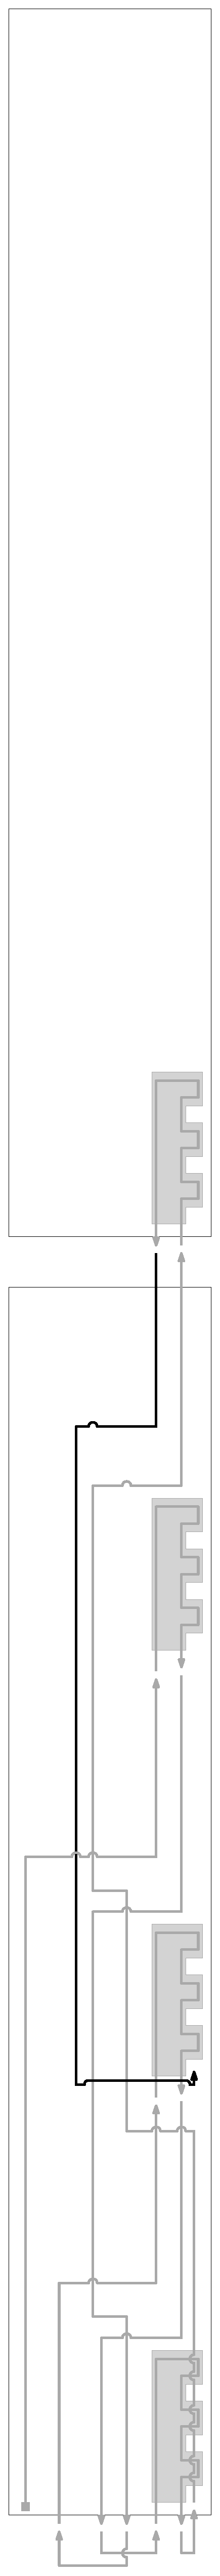
\includegraphics[width=.5in,valign=t]{mid_level_timeline_phase_6}
        \caption{\label{fig:mid_level_timeline_phase_6} Return from ${\mathcal{D}_1}'$ down to ${\mathcal{D}_2}$ }
    \end{subfigure}%
   ~
    \begin{subfigure}[t]{0.14\textwidth}
        \centering
        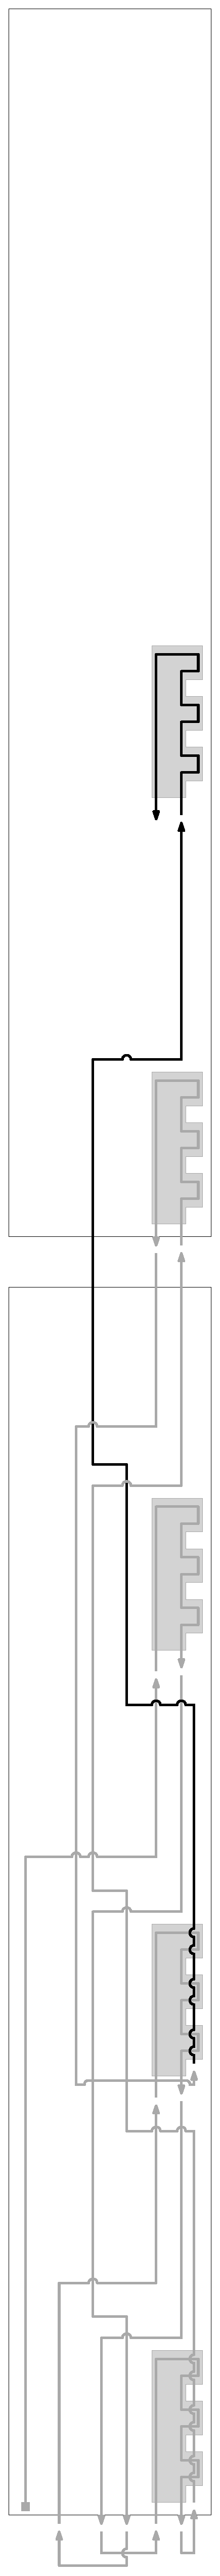
\includegraphics[width=.5in,valign=t]{mid_level_timeline_phase_7}
        \caption{\label{fig:mid_level_timeline_phase_7} The counter reads ${\mathcal{D}_2}$, then writes ${\mathcal{D}_2}'$ }
    \end{subfigure}%
    ~
    \begin{subfigure}[t]{0.14\textwidth}
        \centering
        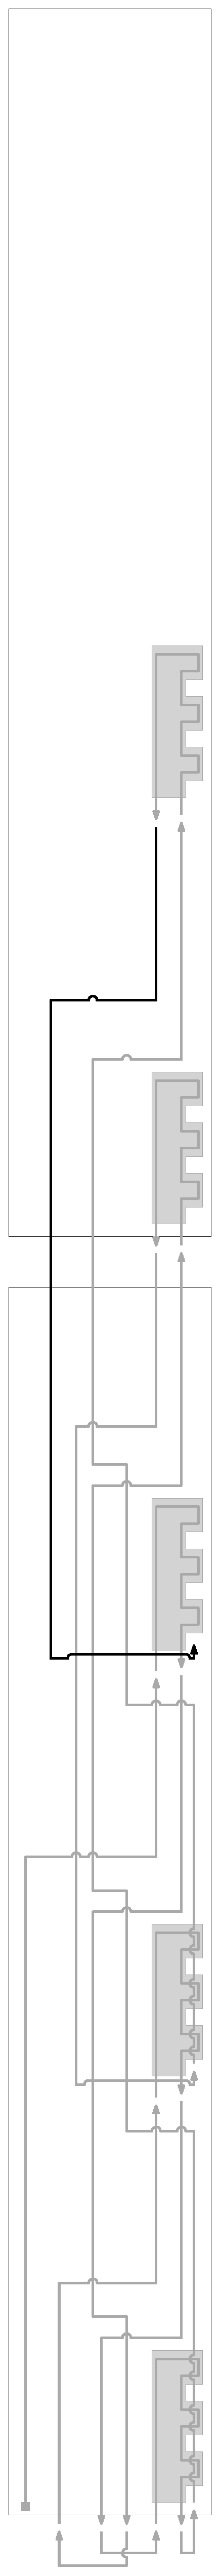
\includegraphics[width=.5in,valign=t]{mid_level_timeline_phase_8}
        \caption{\label{fig:mid_level_timeline_phase_8} Return from ${\mathcal{D}_2}'$ down to ${\mathcal{D}_3}$ }
    \end{subfigure}
    ~
    \begin{subfigure}[t]{0.14\textwidth}
        \centering
        \includegraphics[width=.5in,valign=t]{mid_level_timeline_phase_9}
        \caption{\label{fig:mid_level_timeline_phase_9} The counter reads ${\mathcal{D}_3}$, then writes ${\mathcal{D}_3}'$ }
    \end{subfigure}
    ~
    \begin{subfigure}[t]{0.14\textwidth}
        \centering
        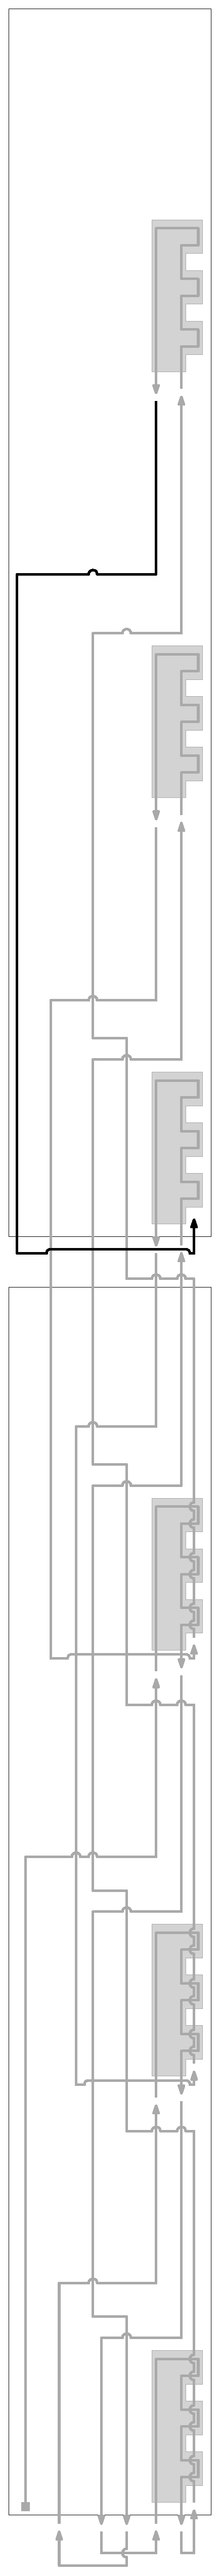
\includegraphics[width=.5in,valign=t]{mid_level_timeline_phase_10}
        \caption{\label{fig:mid_level_timeline_phase_10} Return from ${\mathcal{D}_3}'$ down to ${\mathcal{D}_1}'$ }
    \end{subfigure}


    \caption{\label{fig:mid_level_timeline_overview} An overview that showcases how a digit region is read and written in the next
    counter row.  }

\end{figure}



% Case 1

\begin{figure}
    \centering

    \begin{subfigure}[t]{0.14\textwidth}
        \centering
        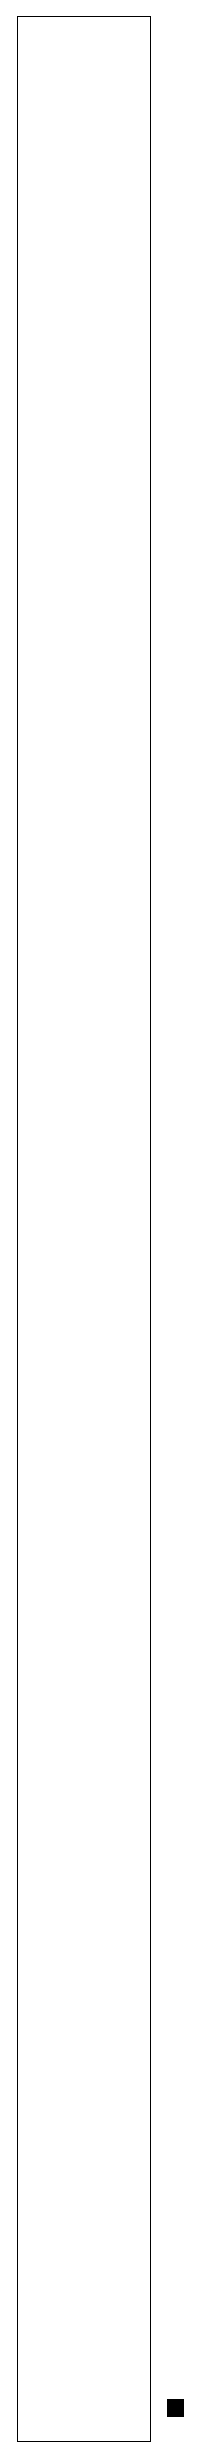
\includegraphics[width=.45in,valign=t]{mid_level_1digit_msr_phase_1}
        \caption{\label{fig:mid_level_1digit_msr_phase_1} Seed tile is placed }
    \end{subfigure} %
    ~
    \begin{subfigure}[t]{0.14\textwidth}
        \centering
        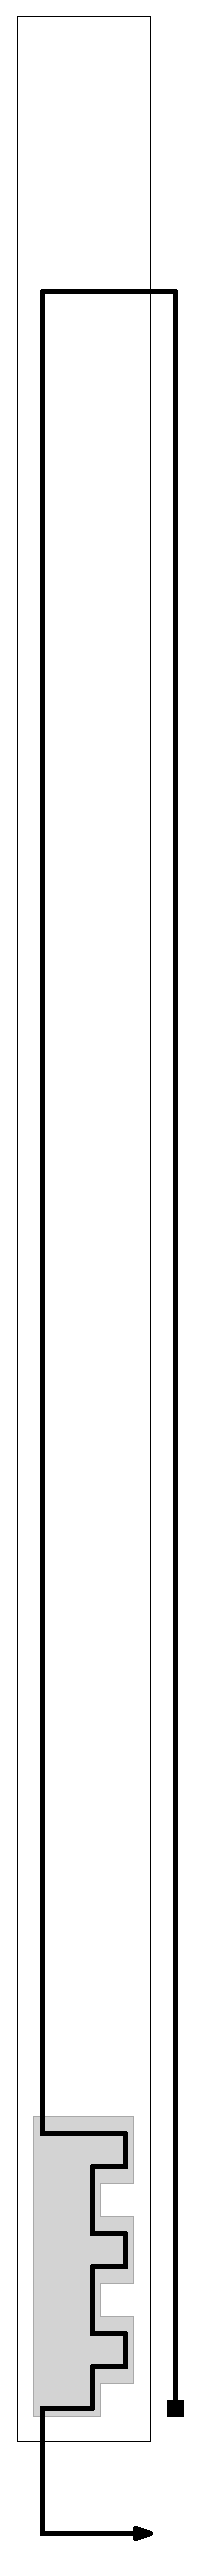
\includegraphics[width=.45in,valign=t]{mid_level_1digit_msr_phase_2}
        \caption{\label{fig:mid_level_1digit_msr_phase_2} Digit 1 is written. }
    \end{subfigure}%
   ~
    \caption{\label{fig:mid_level_1digit_msr_overview} Middle-level overview showcasing how a MSR in case 1 is assembled.  }
\end{figure}

\begin{figure}
    \centering

    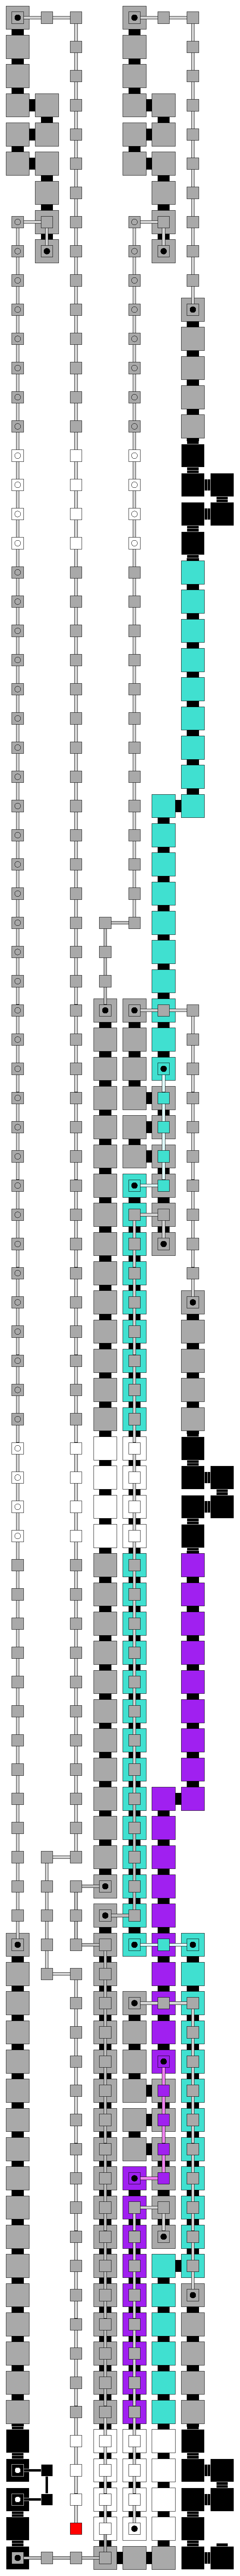
\includegraphics[width=.7in,valign=t]{1digit_msr_seed}

    \caption{\label{fig:1digit_msr_seed} Low-level overview of the MSR in case 1, along with a standard 3 digit region to its east. }

\end{figure}



% Case 2

\begin{figure}
    \centering

    \begin{subfigure}[t]{0.3\textwidth}
        \centering
        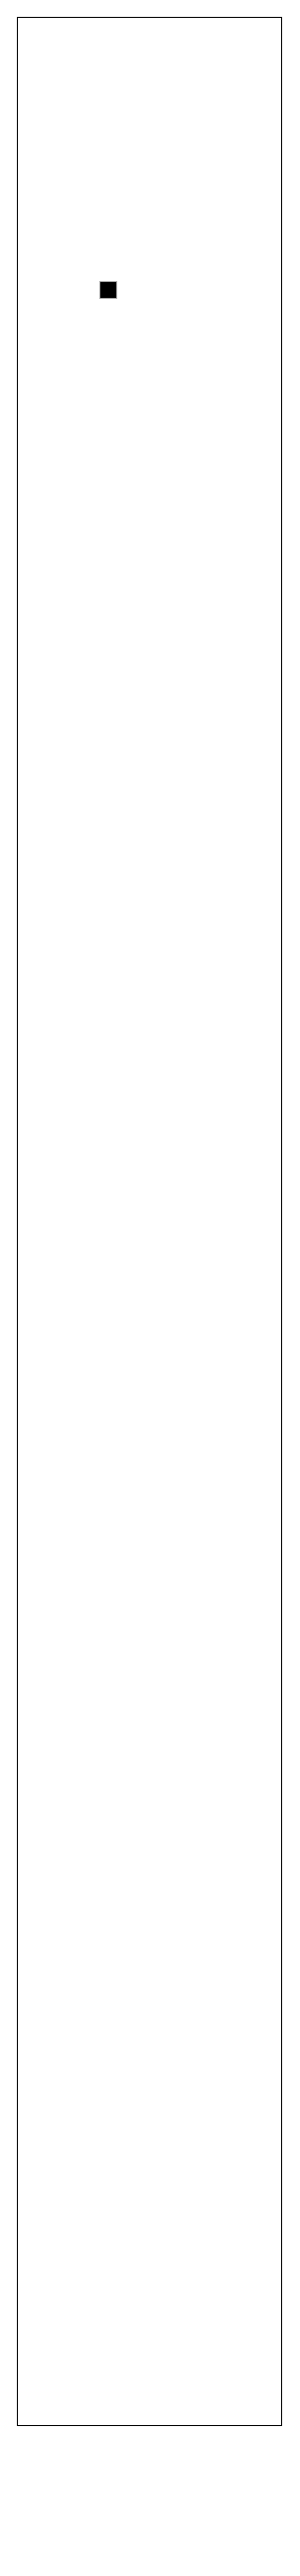
\includegraphics[width=.5in,valign=t]{mid_level_2digit_msr_phase_1}
        \caption{\label{fig:mid_level_2digit_msr_phase_1} Seed tile is placed }
    \end{subfigure} %
    ~
    \begin{subfigure}[t]{0.3\textwidth}
        \centering
        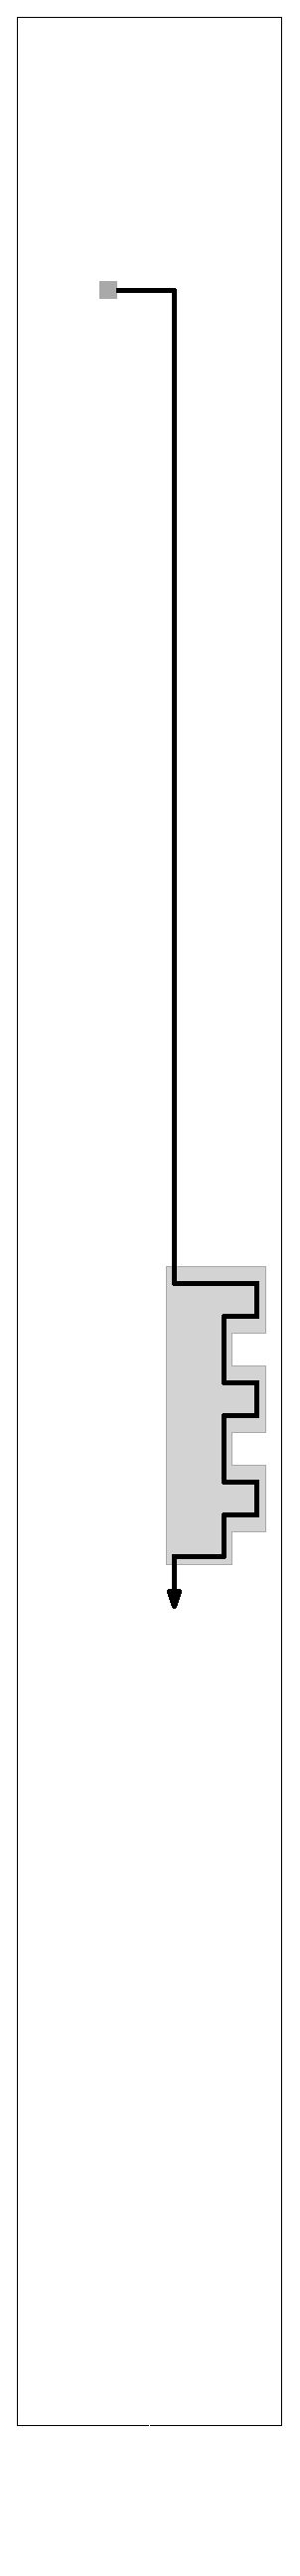
\includegraphics[width=.5in,valign=t]{mid_level_2digit_msr_phase_2}
        \caption{\label{fig:mid_level_2digit_msr_phase_2} Digit 1 is written. }
    \end{subfigure}%
   ~
    \begin{subfigure}[t]{0.3\textwidth}
        \centering
        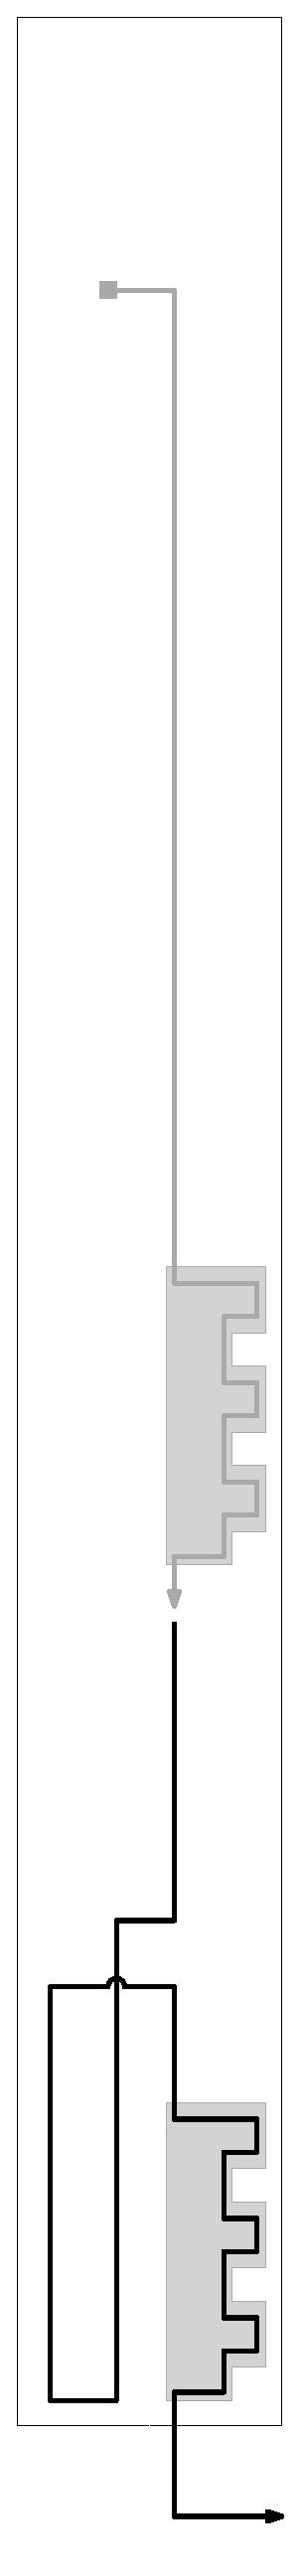
\includegraphics[width=.5in,valign=t]{mid_level_2digit_msr_phase_3}
        \caption{\label{fig:mid_level_2digit_msr_phase_3} Digit 2 is written. }
    \end{subfigure}%
    ~

    \caption{\label{fig:mid_level_2digit_msr_overview} Middle-level overview showcasing how a MSR in case 2 is assembled. }

\end{figure}

\begin{figure}
    \centering

    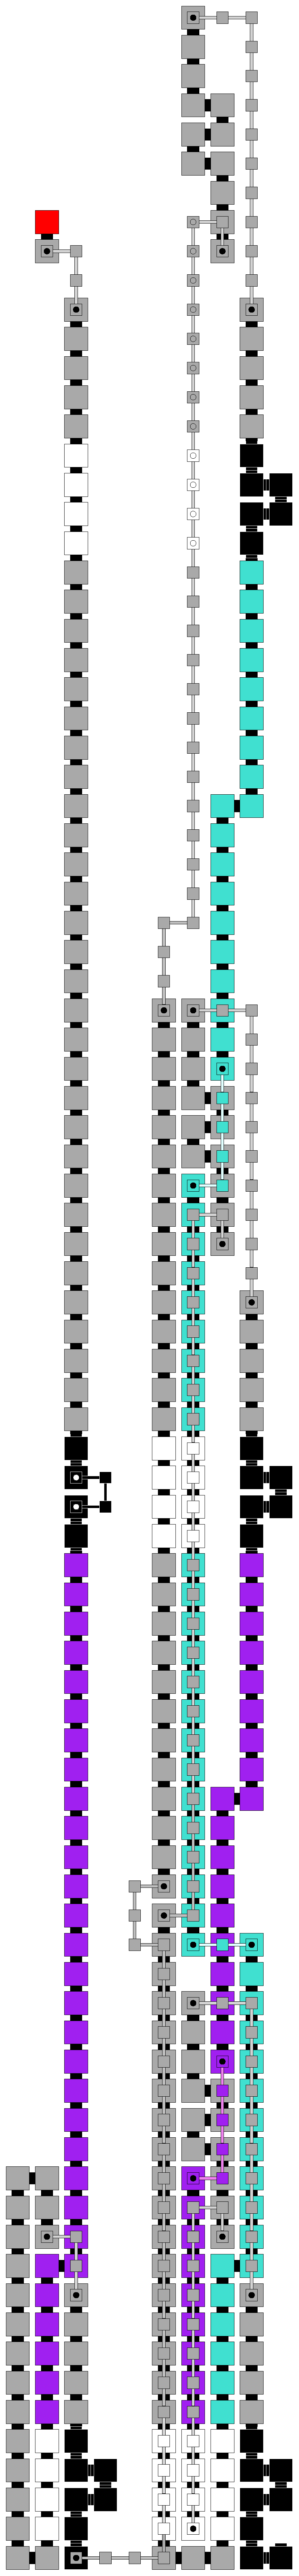
\includegraphics[width=.5in,valign=t]{2digit_msr_seed}

    \caption{\label{fig:2digit_msr_seed} Low-level overview of the MSR in case 2, along with a standard 3 digit region to its east.}

\end{figure}



% Case 3

\begin{figure}
    \centering

    \begin{subfigure}[t]{0.23\textwidth}
        \centering
        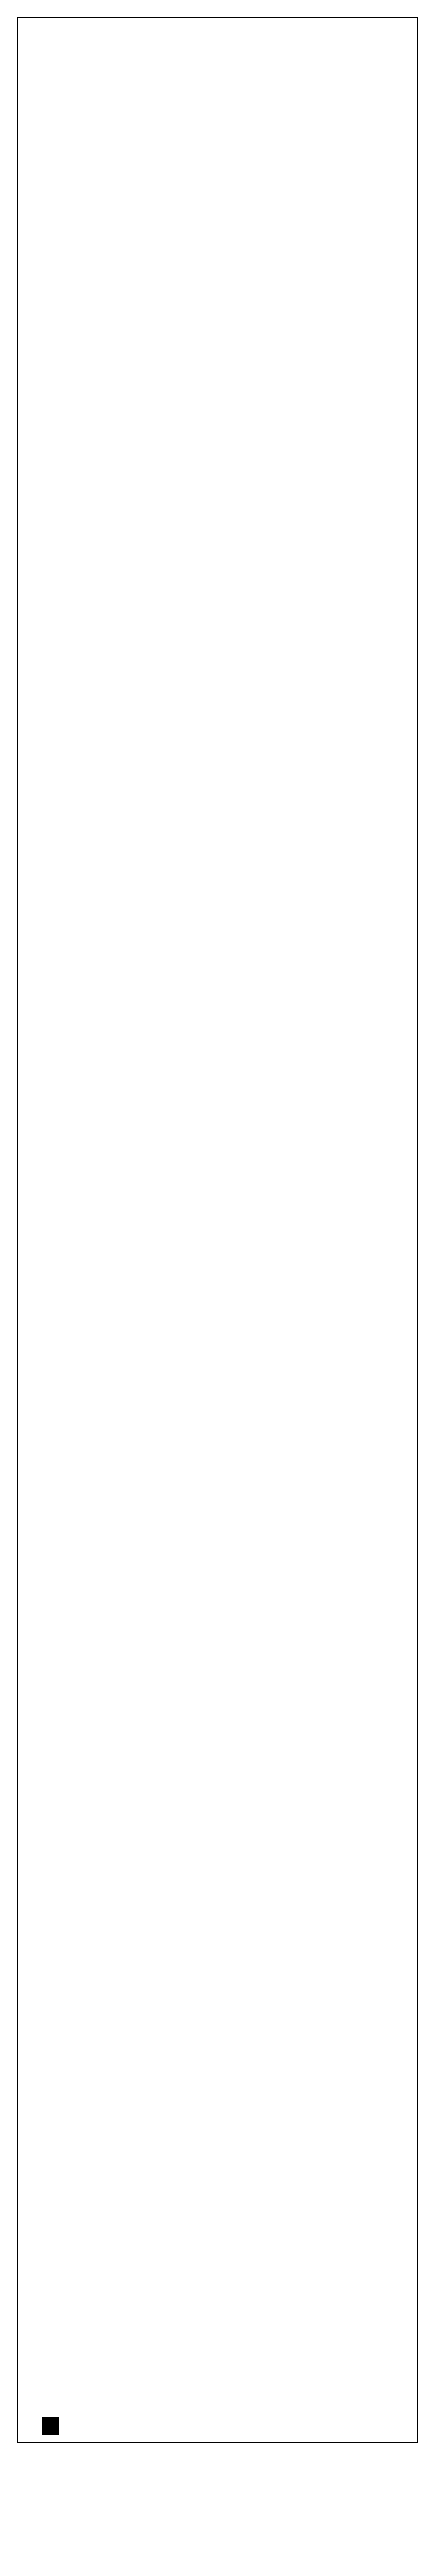
\includegraphics[width=.85in,valign=t]{mid_level_timeline_phase_1}
        \caption{\label{fig:mid_level_timeline_phase_1} Seed tile is placed. }
    \end{subfigure} %
    ~
    \begin{subfigure}[t]{0.23\textwidth}
        \centering
        \includegraphics[width=.85in,valign=t]{mid_level_timeline_phase_2}
        \caption{\label{fig:mid_level_timeline_phase_2} Digit 3 is written }
    \end{subfigure}%
   ~
    \begin{subfigure}[t]{0.23\textwidth}
        \centering
        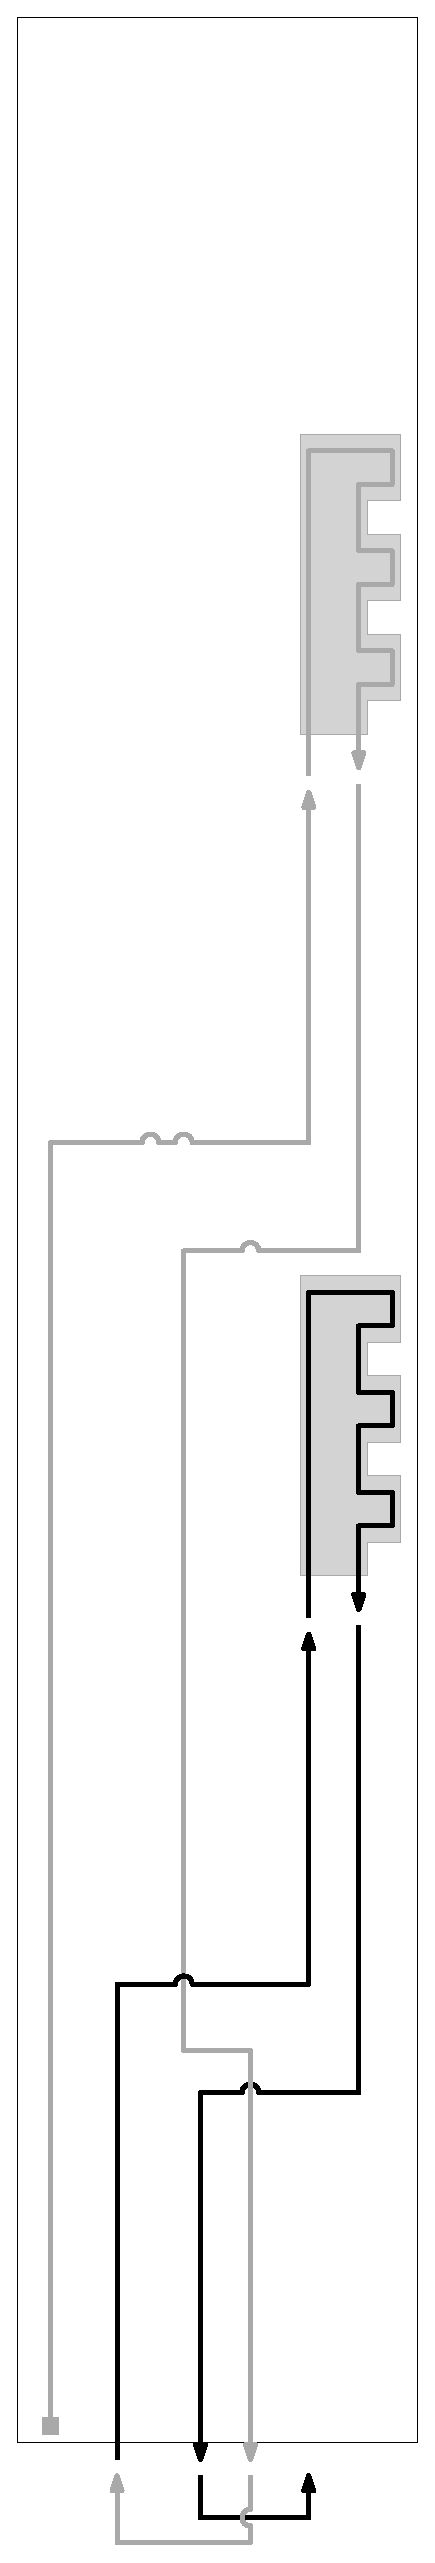
\includegraphics[width=.85in,valign=t]{mid_level_timeline_phase_3}
        \caption{\label{fig:mid_level_timeline_phase_3} Digit 2 is written }
    \end{subfigure}%
    ~
    \begin{subfigure}[t]{0.23\textwidth}
        \centering
        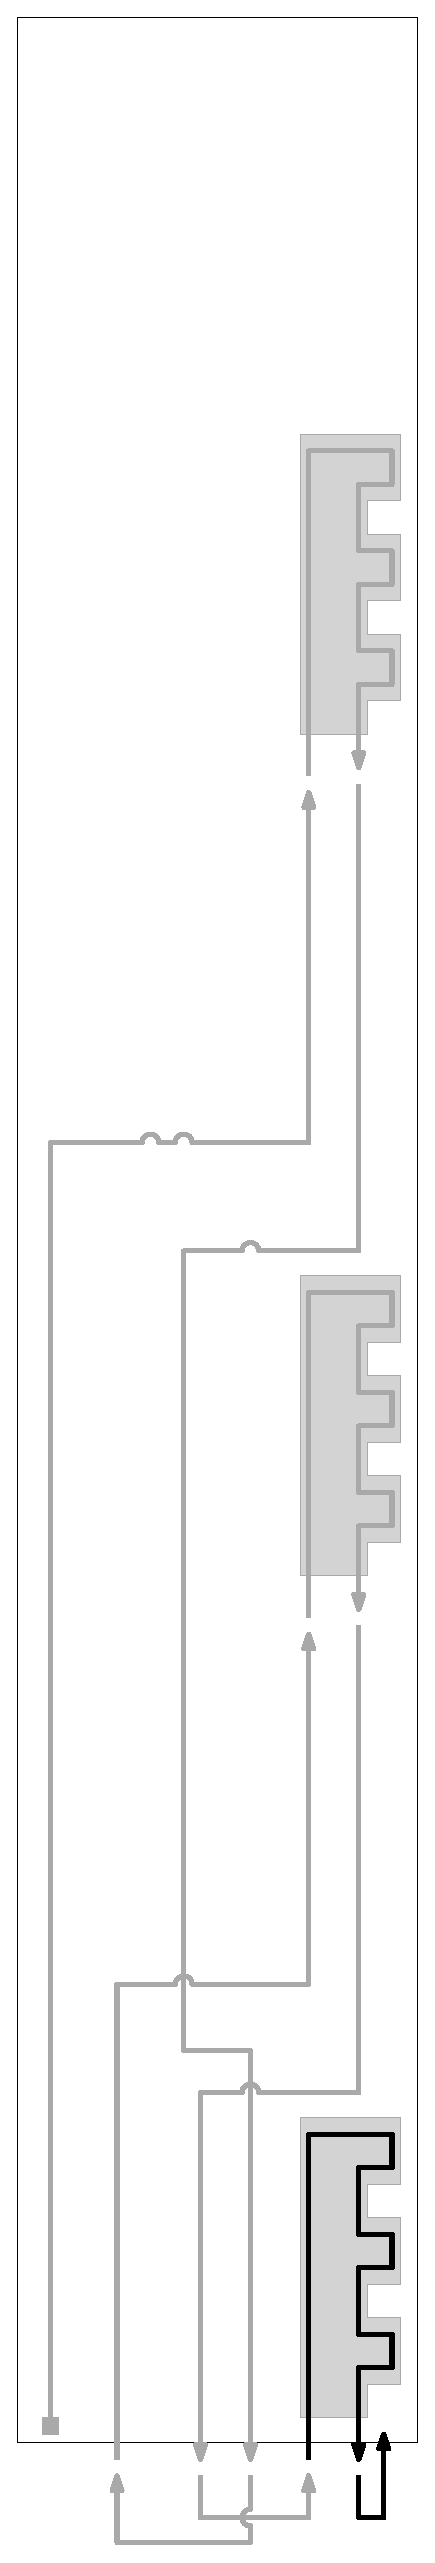
\includegraphics[width=.85in,valign=t]{mid_level_timeline_phase_4}
        \caption{\label{fig:mid_level_timeline_phase_4} Digit 1 is written }
    \end{subfigure}

    \caption{\label{fig:mid_level_timeline_overview} Middle-level overview of how a digit region in the seed is assembled. In the seed, the path is reversed, the digits are written in order of most signifcant to least significant. }
\end{figure}


\begin{figure}
    \centering

    \includegraphics[width=.5in,valign=t]{3digit_msr_seed}

    \caption{\label{fig:3digit_msr_seed} Low-level overview of the MSR in case 3, along with a standard 3 digit region to its east.}
\end{figure}

\end{document}

